\chapter{Cluster Analysys}
\label{ch:cluster}

    In questo capitolo si descriveranno le attività svolte per realizzare dei \textit{clustering} sulle versioni ad attributi continui dei data set prodotti nella fase di \textit{preprocessing} (descritta nel Capitolo \ref{ch:prepr}).

\section{Introduzione alla Cluster Analysys}

    Volendo spendere poche parole per delineare un quadro generale e impiegando una massiccia astrazione dai dettagli, possiamo descrivere un \textit{clustering} come segue, citando direttamente da \cite{clustering}:\\

    "Il \textbf{clustering} o \textbf{analisi dei gruppi} (dal termine inglese \textit{cluster analysis} introdotto da Robert Tryon nel 1939) è un insieme di tecniche di analisi multivariata dei dati volte alla selezione e raggruppamento di elementi omogenei in un insieme di dati."\\

    Volendo sintetizzare ulteriormente questi concetti, si può dire che un \textit{clustering} su di un certo data set è un raggruppamento di istanze \textbf{simili fra loro}. Citando sempre da \cite{clustering}:\\

    "Le tecniche di clustering si basano su misure relative alla somiglianza tra gli elementi. In molti approcci questa similarità, o meglio, dissimilarità, è concepita in termini di distanza in uno spazio multidimensionale. La bontà delle analisi ottenute dagli algoritmi di clustering dipende molto dalla scelta della metrica, e quindi da come è calcolata la distanza. Gli algoritmi di clustering raggruppano gli elementi sulla base della loro distanza reciproca, e quindi l'appartenenza o meno ad un insieme dipende da quanto l'elemento preso in esame è distante dall'insieme stesso."\\

    Questa breve ma efficace descrizione sommaria fornisce già una sufficiente infarinatura riguardo al tipo di azioni da compiere per ottenere un \textit{clustering}: si tratta infatti di cercare all'interno dei data set in esame dei gruppi di istanze simili fra di loro per qualche criterio --- che vedremo essere delle metriche di distanza in uno spazio multidimensionale definito dagli attributi dei dati.\\

    Quanto scritto può essere sufficiente per delineare il quadro generale nel quale si è operato per compiere i passi descritti successivamente. Ovviamente, una trattazione esaustiva sull'argomento necessiterebbe ben altro spazio di quello che si può dedicare in questa tesi di laurea, perciò si rimanda alla consultazione di \cite{dispense} per ulteriori dettagli, qualora quanto sopra riportato non dovesse essere sufficiente per la comprensione di quanto seguirà.

\section{Algoritmi di Clustering}

    La realizzazione di un \textit{clustering} su dei \textit{big data} è ovviamente una di quelle attività che hanno bisogno di essere delegate a un algoritmo per essere eseguite. Si descriveranno in questa sezione alcuni dei più efficaci algoritmi di \textit{clustering} e le implementazioni di Weka.

    \subsection{Algoritmo K-Means}

        Uno dei più noti algoritmi di \textit{clustering} che consente di imporre a priori il numero di \textit{cluster} cercati è senza dubbio \textbf{K-Means}. Come si può leggere in \cite{dispense}:\\

        "The K-means clustering technique is simple [...]. We first choose \textit{K} initial centroids, where \textit{K} is a user-specified parameter, namely, the number of clusters desired. Each point is then assigned to the closest centroid, and each collection of points assigned to a centroid is a cluster. The centroid of each cluster is then updated based on the points assigned to the cluster. We repeat the assignment and update steps until no point changes clusters, or equivalently, until the centroids remain the same." \\

        Il che significa, traducendo e parafrasando:\\

        "La tecnica K-Means è semplice: scegliamo inizialmente \textit{K} centroidi iniziali, dove \textit{K} è il numero di cluster desiderati. Ogni punto del data set è assegnato al centroide più vicino, e ogni collezione di punti assegnati a un centrode è un cluster. Il centroide di ogni cluster viene poi ricalcolato, basandosi sui punti che gli sono stati assegnati. Si ripetono questi passi fino a che nessun punto cambia cluster, o i centroidi non cambiano."\\

        Quindi, si tratta di una procedura iterativa che, a partire da un numero fissato di punti iniziali, chiamati centroidi, migliora ad ogni passo gli assegnamenti fino a che non si raggiunge una situazione di stabilità. \\

        Le librerie di Weka mettono a disposizione un'implementazione di K-Means, che permette di configurare un gran numero di parametri (come si può vedere in Figura \ref{kmeans_weka}).

        \begin{figure}
            \centering
            \caption{finestra che mostra i parametri impostabili dell'algoritmo K-Means}
            \label{kmeans_weka}
            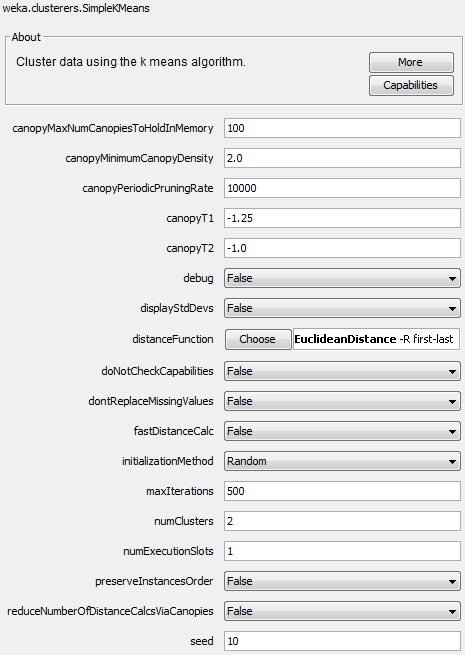
\includegraphics[scale=0.90]{img/cluster_k_means.png}
        \end{figure}

    \subsection{Algoritmo DBSCAN}

        Una algoritmo sostanzialmente diverso dal precedente è DBSCAN, che non si basa sul minimizzare le distanze dal centroide del \textit{cluster}, ma bensì sul raggruppare le istanze del data set in base alla loro \textbf{densità}. \\

        Un'informale ma potente descrizione di questo si può leggere in \cite{dispense}:

        "Density-based clustering locates regions of high density that are separated from one another by regions of low density. DBSCAN is a simple and effective density-based clustering algorithm [...]"\\

        Che tradotto significa:\\

        "Le teniche di clustering basate sulla densità individuano regioni dense separate le une dalle altre da regioni meno dense. DBSCAN è un algoritmo di clustering basato sulla densità semplice ed efficace."\\

        Quindi, si può dire che DBSCAN sia un algoritmo che, a differenza di K-Means, non cerca di individuare a quale dei cluster decisi inizialmente appartenga una data istanza, ma individua invece i cluster "naturali" del data set basandosi sulla densità di istanze nelle varie regioni dello spazio multidimensionali definito dagli attributi. \\

        L'implementazione di DBSCAN fornita da Weka, come si può vedere in Figura \ref{dbscan_weka}, è molto basilare, ma totalmente funzionale.

        \begin{figure}
            \centering
            \caption{finestra che mostra i parametri impostabili dell'implementazione di DBSCAN su Weka}
            \label{dbscan_weka}
            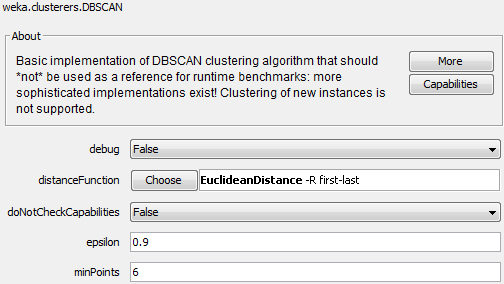
\includegraphics[scale=0.70]{img/dbscan_weka.png}
        \end{figure}

\section{Clustering sulle Valutazioni dei Corsi}

    Una prima serie di tentativi di \textit{cluster analysis} è stata fatta sul data set condensato delle valutazioni dei corsi, utilizzando l'algoritmo K-Means. \\

    Si è ben coscienti che un'analisi di questo tipo su un data set che contiene solo sette elementi \textit{generalmente} non avrebbe molto senso, ma in questo caso si può considerare come un approfondimento della fase di \textit{data understanding} su questo data set.

    \subsection{Lancio di K-Means}

        Adottando un metodo empirico di \textit{trial-and-error}, sono state effettuati innumerevoli lanci di K-Means variando di volta in volta i parametri di input. \\

        Quella che segue è la configurazione che genera il miglior risultato ottenuto:

        \begin{center}
            \texttt{weka.clusterers.SimpleKMeans -init 0 -max-candidates 100 -periodic-pruning 10000 -min-density 2.0 -t1 -1.25 -t2 -1.0 -V -M -N 2 -A "weka.core.EuclideanDistance -R first-last" -I 5000 -num-slots 1 -S 997}
        \end{center}

        Nonostante l'elevato numero di parametri a disposizione, in realtà soltanto alcuni hanno influenzato il risultato finale:

        \begin{itemize}
            \item come metrica è stata scelta la \textbf{distanza Euclidea}\footnote{Si tratta di una metrica che misura la distanza fra due punti di uno spazio multidimensionale come la lunghezza del segmento che li unisce.};
            \item sono stati imposti due centroidi iniziali scelti casualmente, ottenendo pertanto un partizionamento con due cluster
        \end{itemize}

        Ai fini del clustering, sono stati considerati soltanto tre attributi: la valutazione complessiva del corso, la deviazione standard delle valutazioni e la percentuali di valutazioni sufficienti.

        \lstinputlisting[caption={Output della console di Weka relativo al lancio di K-Means sul data set delle valutazioni dei corsi}]{../cluster/eval_kmeans.txt}

        \begin{figure}
            \centering
            \caption{sezione dello spazio di esistenza del data set delle valutazione dei corsi lungo il piano definito da "valutazione complessiva" e "percentuale di valutazioni sufficienti", con evidenziato per ogni istanza il cluster di appartenenza}
            \label{eval_kmeans}
            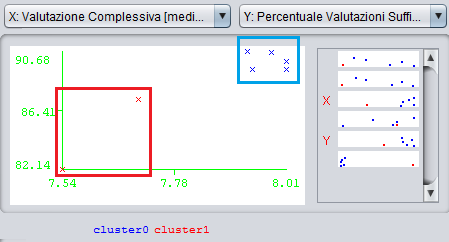
\includegraphics[scale=1.2]{../cluster/eval_kmeans.png}
        \end{figure}

        Come si può vedere dalla Figura \ref{eval_kmeans}, il data set è stato diviso in due cluster che appaiono visivamente ben separati.

        \begin{itemize}
            \item \textbf{Cluster 1} (rosso): A. A. 2013-2014 e 2010-2011
            \item \textbf{Cluster $0$} (blu): gli altri cinque A. A.
        \end{itemize}

\section{Clustering sulla join dei due data set}

    Quanto segue è la parte fondamentale di questa \textit{cluster analysis}, ovvero lo studio della versione ad attributi continui dell'unione dei due data set iniziali.

    \subsection{Lancio di K-Means}

        In modo del tutto analogo a quanto fatto per la precedente attività di clustering, sono state fatte molte prove al fine di raggiungere una configurazione di lancio di K-Means soddisfacente: \\

        \lstinputlisting[caption={Output della console di Weka relativo al lancio di K-Means sul data set risultante dal join delle due collezioni di dati a disposizione}]{../cluster/min_kmeans_2cl.txt}

        Occorre notare varie cose, al fine di comprendere il signficato di quanto è stato ottenuto:

        \begin{itemize}
            \item la \textbf{somma dell'errore quadratico}\footnote{Si tratta di una metrica che da una misura di quanto i punti che compongono il cluster siano distanti dal centroide --- in parole estremamente semplici: più è alto, più il cluster è composto da punti sparsi.} all'interno dei cluster è molto maggiore di quella ottenuta nell'occasione precedente, ma non si può assolutamente fare un confronto diretto fra le due quantità, sia per la diversa natura dell'indagine che per il diverso numero di istanze tenute in considerazione;
            \item al fine di semplificare il significato geometrico della metrica di distanza scelta (quella Euclidea), sono stati presi in considerazione ai fini del clustering soltanto gli attributi più caratterizzanti del dataset:
                \subitem --- Voto medio degli studenti
                \subitem --- Ritardo medio degli studenti
                \subitem --- Valutazione media del corso
            \item sono stati cercati, anche in questo caso, due soli cluster; semanticamente, si può intendere di voler dividere i corsi "migliori", quelli che hanno ricevuto delle buone valutazioni e in cui gli studenti hanno prodotto delle buone performance, da quelli "peggiori".
        \end{itemize}

    \subsection{Analisi dei risultati di K-Means}

        \begin{figure}
            \centering
            \caption{matrice di prossimità, matrice di incidenza e correlazione fra di esse per misurare la contà del clustering effettuato con K-Means}
            \label{matricidistanze}
            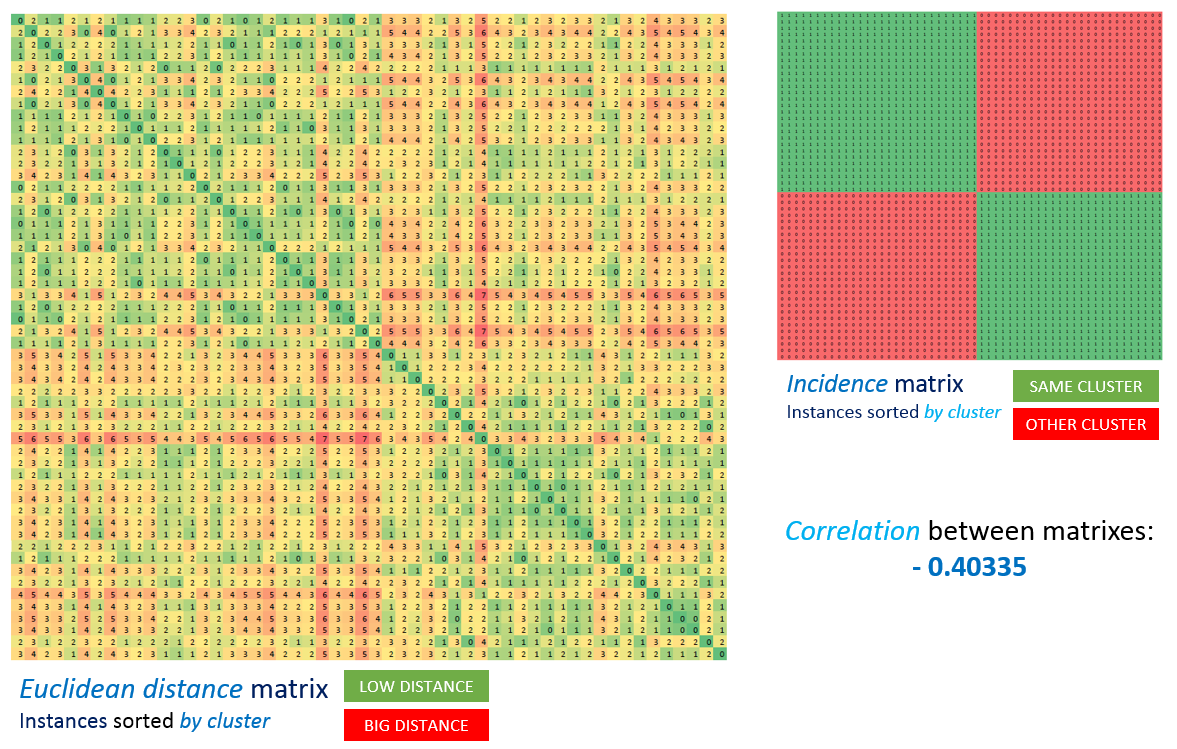
\includegraphics[scale=0.32]{../pres/cluster5.png}
        \end{figure}

        Da un punto di vista tecnico, la bontà del risultato può essere misurata con la correlazione fra la \textit{matrice di incidenza} e la \textit{matrice di prossimità}: un valore negativo indica una tendenza delle distanze fra i punti dello stesso cluster ad essere minore di quelle fra punti di cluster diversi. Come si può vedere in Figura \ref{matricidistanze}, nel caso di questo specifico clustering la correlazione fra le due matrici è circa $-0.4$, il che indica i cluster ottenuti sono abbastanza separati. \\

        Il risultato ottenuto è parzialmente in linea con l'intento che ci si era prefissati. Il cluster identificato da Weka come \textbf{Cluster $0$}, e colorato di \textbf{blu} nei grafici che verranno mostrati, può essere considerato quello dei corsi migliori. Conseguentemente, il \textit{cluster 1} può essere letto come quello dei corsi peggiori rispetto agli altri e rispetto alle metriche considerate. \\

        Si vada innanzitutto a vedere come sono state raggruppate le istanze del data set nei due cluster, rispetto ai tre attributi caratterizzati (Figure \ref{1}, \ref{2} e \ref{3}). Come si può agilmente notare, la divisione che ci si aspettava di vedere è presente.\\

        \begin{figure}
            \centering
            \caption{sezione dello spazio di esistenza del data set delle valutazione dei corsi lungo il piano definito da "voto medio" e "ritardo medio", con evidenziato per ogni istanza il cluster di appartenenza}
            \label{1}
            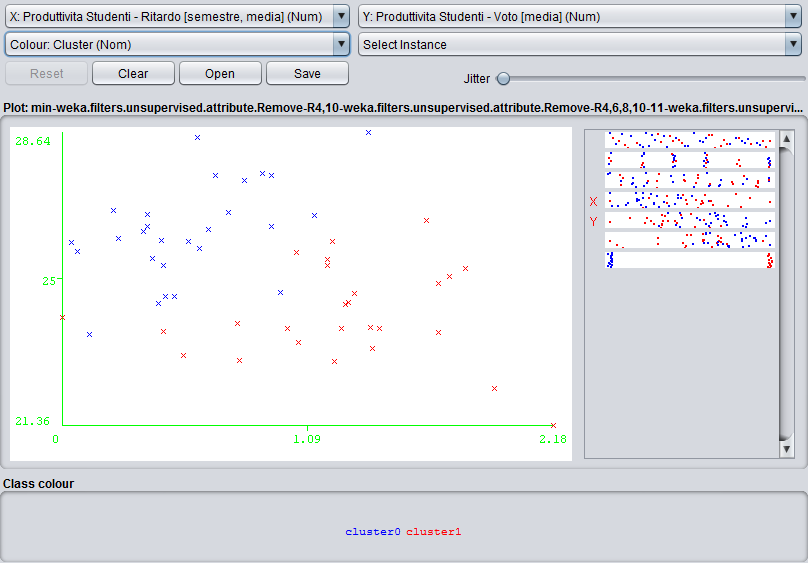
\includegraphics[scale=0.5]{../cluster/min_kmeans_2cl_attr1.png}
        \end{figure}

        \begin{figure}
            \centering
            \caption{sezione dello spazio di esistenza del data set delle valutazione dei corsi lungo il piano definito da "ritardo medio" e "valutazione della didattica", con evidenziato per ogni istanza il cluster di appartenenza}
            \label{2}
            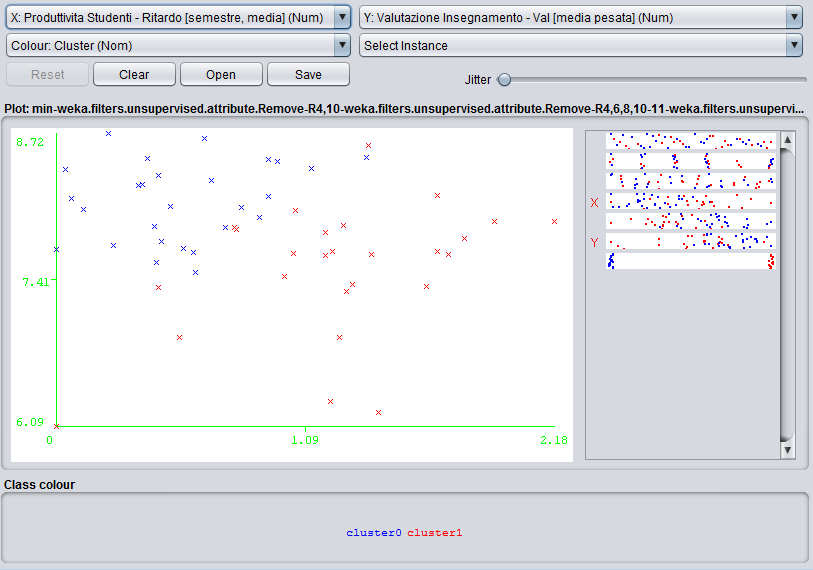
\includegraphics[scale=0.5]{../cluster/min_kmeans_2cl_attr2.png}
        \end{figure}

        \begin{figure}
            \centering
            \caption{sezione dello spazio di esistenza del data set delle valutazione dei corsi lungo il piano definito da "voto medio" e "valutazione della didattica", con evidenziato per ogni istanza il cluster di appartenenza}
            \label{3}
            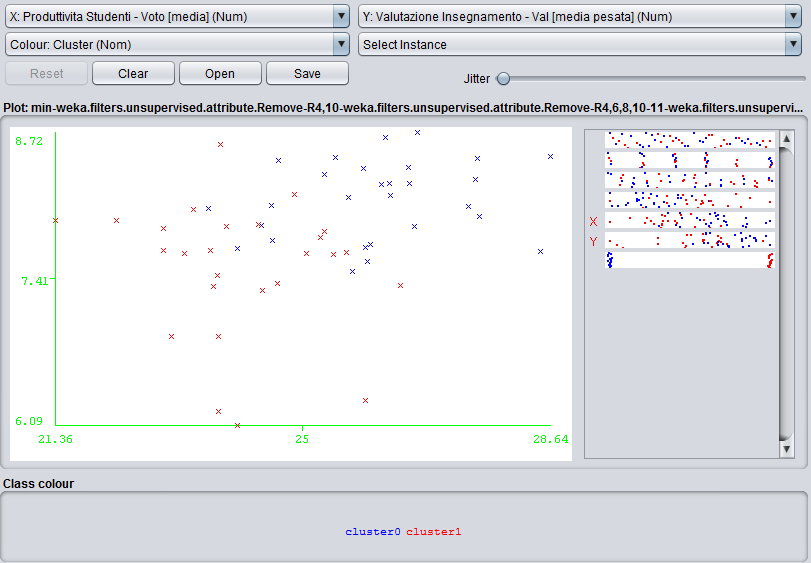
\includegraphics[scale=0.5]{../cluster/min_kmeans_2cl_attr3.png}
        \end{figure}

        Volendo ragionare sulla composizione dei due cluster, si è andati a vedere innanzitutto se l'Anno Accademico di riferimento ha un qualche ruolo nella produzione di questo risultato. Come si può osservare nelle Figure \ref{AA1} e \ref{AA2}, la popolazione di entrambi i cluster è abbastanza simile riguardo a questo aspetto. \\

        \begin{figure}
            \centering
            \caption{composizione del Cluster $0$ riguardo gli Anni Accademici considerati dal data set}
            \label{AA1}
            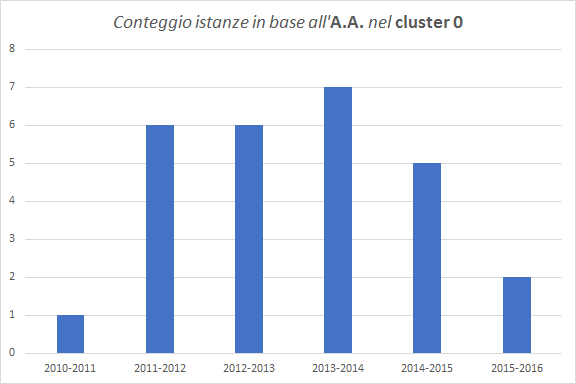
\includegraphics[scale=0.75]{../cluster/min_kmeans_2cl_AA_cl0.png}
        \end{figure}

        \begin{figure}
            \centering
            \caption{composizione del Cluster 1 riguardo gli Anni Accademici considerati dal data set}
            \label{AA2}
            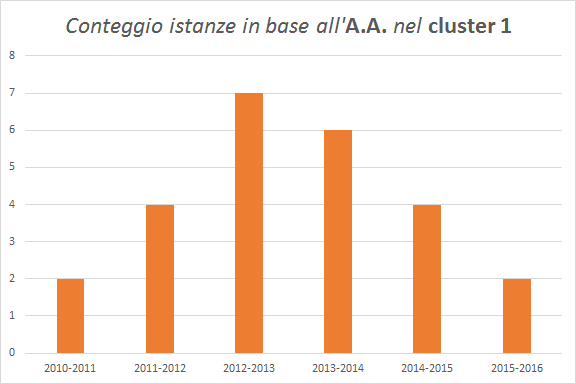
\includegraphics[scale=0.75]{../cluster/min_kmeans_2cl_AA_cl1.png}
        \end{figure}

        Per quanto riguarda invece l'individuare in quale cluster sia finito ogni corso, si è innanzitutto osservata la composizione totale dei due cluster. In caso si fosse trattato di una \textit{cluster analysis} su veri e propri \textit{big data}, questo non sarebbe ovviamente stato possibile, ma dato che il data set in esame ha a malapena sessanta istanze, è stato possibile stilare la seguente lista: \\

        \lstinputlisting{../cluster/min_kmeans_2cl_composition.txt}

        Tuttavia, tale lista non consente di vedere immediatamente alcuna caratteristica fondamentale del clustering in esame. La maggior parte dei corsi, rappresentati da varie istanze secondo l'Anno Accademico di riferimento, è presente sia nel Cluster $0$ che nel Cluster 1. Pertanto, è stata realizzata la tabella mostrata in Figura \ref{tabella} per evidenziare quali corsi di esame sono del tutto assenti da quali cluster.\\

        \begin{figure}
            \centering
            \caption{tabella che mostra la composizione dei cluster in riferimento ai corsi di esame}
            \label{tabella}
            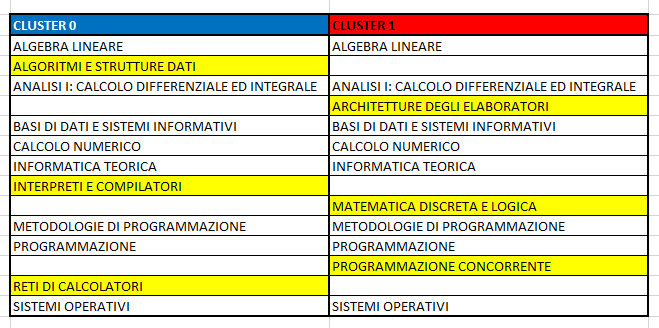
\includegraphics[scale=0.65]{../cluster/min_kmeans_2cl_corsi_cluster.png}
        \end{figure}

        Da tale Figura, si può notare che il Cluster $0$, quello dei corsi "buoni", comprende tutte le istanze relative ai corsi di:

        \begin{itemize}
            \item Algoritmi e Strutture dati
            \item Interpreti e Compilatori
            \item Reti di Calcolatori
        \end{itemize}

        Inoltre, si può vedere che nel Cluster 1, quello dei corsi "meno buoni", sono presenti tutte le istanze dei seguenti corsi:

        \begin{itemize}
            \item Architetture degli Elaboratori
            \item Matematica Discreta e Logica
            \item Programmmazione Concorrente
        \end{itemize}

        Questa caratteristica richiama fortemente quanto visto nel Capitolo \ref{ch:undst}, ovvero durante la fase di \textit{data understanding}, rafforzando quindi l'ipotesi della bontà dell'analisi che si sta effettuando. \\

        Volendo approfondire ulteriormente l'analisi della composizione dei cluster, nelle Figure \ref{eval}, \ref{ritardo} e \ref{voto} si possono vedere degli istogrammi che mostrano la somma dei tre attributi considerati per realizzare il clustering. Ovviamente, i valori assoluti di tali somme non significano niente, ma è interessante vedere come gli attributi "positivi" --- la valutazione della didattica e il voto medio --- hanno una somma più elevata nel Cluster $0$, mentre quello "negativo" --- il ritardo nel dare gli esami --- è molto più accentuato nel Cluster 1.

        \begin{figure}
            \centering
            \caption{istogramma che mostra la somma dell'attributo "valutazione della didattica" nei due cluster ottenuti, divisa per Anno Accademico}
            \label{eval}
            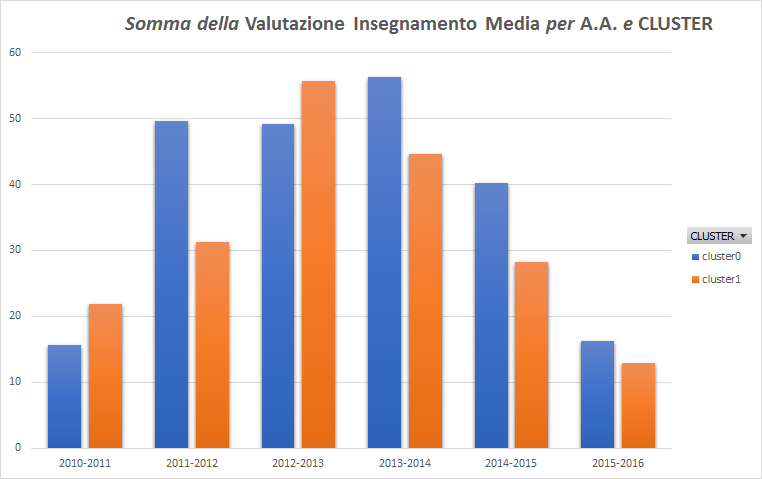
\includegraphics[scale=0.5]{../cluster/min_kmeans_2cl_eval.png}
        \end{figure}

        \begin{figure}
            \centering
            \caption{istogramma che mostra la somma dell'attributo "ritardo medio nel dare gli esami" nei due cluster ottenuti, divisa per Anno Accademico}
            \label{ritardo}
            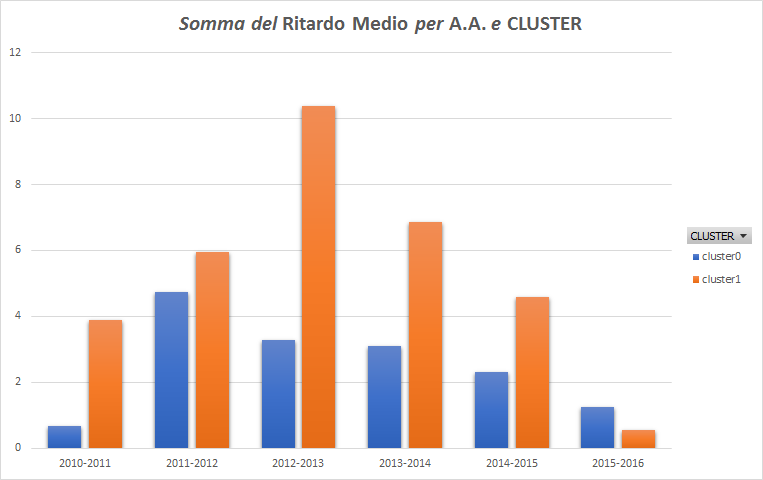
\includegraphics[scale=0.5]{../cluster/min_kmeans_2cl_ritardo.png}
        \end{figure}

        \begin{figure}
            \centering
            \caption{istogramma che mostra la somma dell'attributo "voto medio conseguito negli esami di profitto" nei due cluster ottenuti, divisa per Anno Accademico}
            \label{voto}
            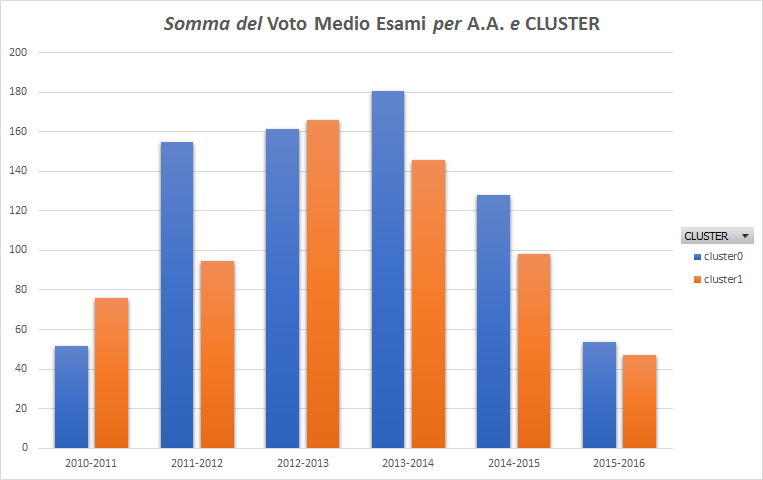
\includegraphics[scale=0.5]{../cluster/min_kmeans_2cl_voto.png}
        \end{figure}

    \subsection{Tentativo di utilizzo di DBSCAN}

    Come il titolo di questa sezione suggerisce, non è stato possibile utilizzare con profitto l'algoritmo DBSCAN. \\

    Imitando quanto fatto con K-Means, ovvero limitando il numero di attributi da considerare per il clustering, ci si aspetterebbe che un algoritmo basato sulla densità possa esibire delle buone performance. Per facilitare ulteriormente l'esecuzione di DBSCAN, è stato addirittura scartato l'attributo relativo al ritardo degli studenti. Così facendo, si è ottenuto uno spazio bidimensionale in cui l'algoritmo può facilmente operare - e che si presta bene a un'interpretazione visiva. \\

    Invece, non è stato possibile ottenere nessun risultato diverso da un cluster unico, per qualunque valore di epsilon e per qualsiasi numero di punti minimi richiesti. Questo perché evidentemente i punti nel nostro piano di analisi sono addensati tutti in un'unica regione, fatto che possiamo agilmente verificare osservandone un grafico in Figura \ref{dbscan}.

    \begin{figure}
        \centering
        \caption{piano composto dalle dimensioni "Voto Medio negli Esami" e "Valutazione Media dell'Insegnamento", sul quale è stato tentato il clustering con l'algoritmo DBSCAN}
        \label{dbscan}
        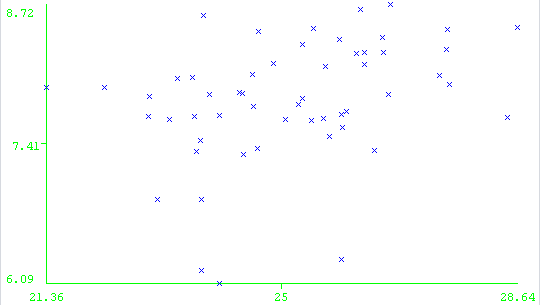
\includegraphics[scale=0.80]{../cluster/dbscan.png}
    \end{figure}